\documentclass[tikz, border=5pt]{standalone}

% Required packages
\usepackage{pgfplots}
\usepackage{pgfplotstable}
\usepackage{tikzviolinplots}
\pgfplotsset{compat=1.18}

\usepackage{cite}
\usepackage{amsmath,amssymb,amsfonts}
\usepackage{algorithmic}
\usepackage{graphicx}
\usepackage{textcomp}
\usepackage{xcolor}
\usepackage{tikz}
\usepackage{physics}
\usepackage{algorithm}
\usepackage{pgfplots}
\usepackage{pgfplotstable}
% \usepackage[sorting=none]{biblatex}
\usepgfplotslibrary{statistics}
\usepackage{etoolbox} % for \ifnumcomp
\usepackage{listofitems} % for \readlist to create arrays
% \usepackage[ruled,vlined]{algorithm% Increase row height
\renewcommand{\arraystretch}{1.4}

% Adjust column spacing
\setlength{\tabcolsep}{8pt}  % default is 6pt, increasing it for better spacing

\tikzset{>=latex} % for LaTeX arrow head
\colorlet{myred}{red!80!black}
\colorlet{myblue}{blue!80!black}
\colorlet{mygreen}{green!60!black}
\colorlet{mydarkred}{myred!40!black}
\colorlet{mydarkblue}{myblue!40!black}
\colorlet{mydarkgreen}{mygreen!40!black}
\tikzstyle{node}=[very thick,circle,draw=myblue,minimum size=22,inner sep=0.5,outer sep=0.6]
\tikzstyle{connect}=[->,thick,mydarkblue,shorten >=1]
\tikzset{ % node styles, numbered for easy mapping with \nstyle
  node 1/.style={node,mydarkgreen,draw=mygreen,fill=mygreen!25},
  node 2/.style={node,mydarkblue,draw=myblue,fill=myblue!20},
  node 3/.style={node,mydarkred,draw=myred,fill=myred!20},
}
\def\nstyle{int(\lay<\Nnodlen?min(2,\lay):3)} % map layer number onto 1, 2, or 3

\usetikzlibrary{arrows.meta,shadows,positioning}
\usetikzlibrary{calc}
\usetikzlibrary{fit, positioning, shapes.geometric}
\tikzset{
	frame/.style={
		rectangle, draw,
		text width=6em, text centered,
		minimum height=4em,drop shadow,fill=white,
		rounded corners,
	},
	line/.style={
		draw, -{Latex},rounded corners=3mm,
	}
}
% Tikz Library
\usetikzlibrary{calc, quotes, angles}
\pgfmathsetmacro{\r}{0.8}
\pgfmathsetmacro{\Phi}{-160}
\pgfmathsetmacro{\Theta}{-90}
\usepackage{fontawesome5}
\usepackage{float}
% \def\BibTeX{{\rm B\kern-.05em{\sc i\kern-.025em b}\kern-.08em
%     T\kern-.1667em\lower.7ex\hbox{E}\kern-.125emX}}








    \begin{document}

% \begin{figure}[H]
% 	\centering
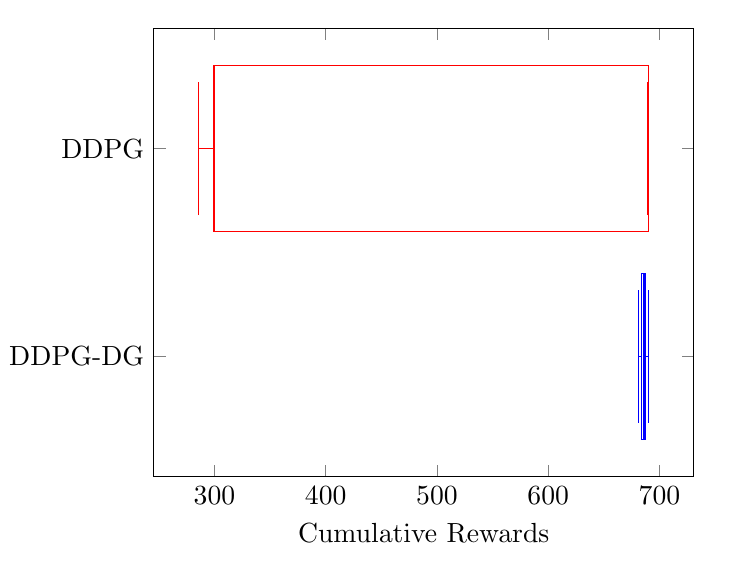
\begin{tikzpicture}
	\hspace{-10pt}
	\begin{axis}
	  [
	  ytick={1,2},
	  yticklabels={DDPG-DG, DDPG},
  xlabel=Cumulative Rewards,
	  ]
	  \addplot+[
boxplot prepared={
lower whisker=681.515208,
lower quartile=683.773397,
median=685.437301,
upper quartile=686.945523,
upper whisker=690.203711
},
		] coordinates {};
	  \addplot+[
		boxplot prepared={
lower whisker=286.00839,
lower quartile=299.609773,
median=689.879372,
upper quartile=690.021882,
upper whisker=689.640044
},
	  ] coordinates {};
	\end{axis}
	% model parameter variation 1000 samples mont carlo
  \end{tikzpicture}
%   \caption{Neural network architecture of the actor in the DDPG algorithm.}
%   \label{fig:actor_nn}
% \end{figure}


\end{document}